\chapter{Evaluation}
\label{cha:evaluation}
% describe experiments:
% - setup
% - number of measurements
% - show results in Figures and/or tables and discuss and compare the results
In this chapter, we evaluate the usability and performance of our system in various experiments. First, we introduce the simulation environment responsible for setting up and running the experiments, the deployment of our system, and some concepts relevant to the evaluation. Afterward, we present simulations and measurements to evaluate the usability and performance of our system. The experiments and results are structured in several sections with different focuses. First, we take a closer look at the end-to-end latency, which is a crucial part of an in-memory system. Then, we present the simulation experiments for different traces, indicating some usability limitations due to the design of our system. An important role is given to the endpoint scheduler, whose performance and decision-making are discussed afterward. This leads to the motivation for burst workloads and why the design of our system is advantageous in this scenario. The related focus on a reactive system leads to a closer discussion and evaluation of the reactivity of our system using the serverless platform. 

~\\
For each section in the evaluation, we first give an overview of the experiment, followed by a discussion and their results. A summary highlights the experiment's findings at each section's end. The next Chapter~\ref{cha:discussion_and_outlook} provides a general summary of the evaluation in terms of the usability of our system. Appendix Table~\ref{tab:costs} provides detailed information for each simulation used to derive the total costs in our evaluations. 

\section{Setup}
\label{sec:setup}
% include relevant details for the evaluation part written in python
% mention the cloudwatch queries for Lambda
% mention the log file written by the orchestrator for the redis runtime duration
First, we describe how our system is deployed on AWS. Appendix~\ref{sec:aws_setup} provides a more detailed explanation of the deployment and the specific configurations required to get our system up and running, while in this section, we focus more on the actual cloud components and associated costs. Next, we cover the client part of our system, as shown in Figure~\ref{fig:system_overview}, which is the part we simulate in our experiments. Those experiments are based on replaying a trace of requests specified by a time delay in seconds since the start of the simulation. So our simulation environment is responsible for creating a trace of requests, simulating them, and collecting the data needed to evaluate the cost and performance of the simulation. We also introduce an offline endpoint scheduler that knows the trace in advance and can be used to evaluate the performance of our scheduler. To compare the cost of our system, we introduce Redis-based comparison systems and explain what to consider when referring to them.

\subsection{System Deployment}
\label{subsec:system_deployment}
Our system is fully deployed on AWS in the Europe(Frankfurt) region (\code{eu-central-1}). The deployment includes two EC2 instances for hosting the reverse proxy and orchestrator, an additional EC2 instance for the self-hosted Redis caching layer, a Lambda function for the second in-memory caching layer, and an S3 bucket where the desired object is stored. While Appendix~\ref{sec:aws_setup} covers the actual steps to get our system up and running in more detail, in this section, we focus on the component specifications relevant to the evaluation. The EC2 instances are on-demand instances (\code{t2.micro}) with one vCPU and one GiB of memory for \$0.0134 per hour. The AWS Lambda function is configured with 1024 MB of memory and a timeout of four minutes\footnote{This timeout should never be triggered and was established to avoid unnecessary costs during development.}, and uses the Go 1.x runtime and $x86\_64$ instruction set architecture. Other resources such as the CPU for the Lambda function are allocated proportionally to the amount of memory chosen. The use of S3 is not of further interest since we assume that this layer is present in any system we consider.
% While we chose the lowest memory setting for our function to minimize cost during our testing, we will use the price for the AWS Lambda function including 1024 MB of memory for reasons explained in section~\ref{subsec:comparison_systems}.


\subsection{Simulation Environment}
\label{subsec:simulation_environment}
The whole simulation part is written in python and divided into three parts. The first part provides several ways to generate/derive a request trace written to an output file and used by the second step, which executes the requests on the target system. The simulation again generates an output file, which the evaluation step can then use to retrieve more information and display an initial evaluation, which we will discuss in the following sections.

~\\
The environment used for the simulation is a single machine with an Intel Core i7-9700K @3.60GHz CPU with eight cores and 32 GiB RAM running Arch Linux 5.15.16-1-lts. Most simulations were performed for a simple HTML object with size 144B. Thus, if no other specifications are made for the object size, we always use the S3 object of size 144B.

\subsubsection{Trace Generation/Derivation}
In order to run arbitrary simulations on our system and thus model the actual client, we write a standardized trace file for the simulator part. Each line in the trace file contains the information of a request; it includes the time offset from the beginning of the simulation (in seconds), the method of the requests (only \code{get}), and the key for the object to be queried. As shown below, the generation script supports different methods to derive a trace. Depending on the method, multiple additional arguments can be specified:
\begin{itemize}
    \item \textbf{poisson:} This method models the requests for a key as a Poisson Process. It requires an additional argument specifying the $\lambda$ parameter of the Poisson process and indicates the rate of requests per minute. A Poisson process is commonly used to model random arrival times of events that occur with a certain frequency~\cite{noauthor_basic_nodate}. Using a Poisson process makes it easy to derive the arrival times since they are independent and follow a simple exponential distribution with the same argument $\lambda$. Using the Python module \code{random} and its function \code{expovariate}, we can easily derive the arrival times. In this method, we need to specify the total duration of the simulation, so we add arrival times until we exceed the specified duration.
    \item \textbf{spike-simple:} A normal distribution is used to model a spike workload. This method is designed to experiment with different spikes by changing the standard deviation of the normal distribution and the number of samples. The Python module \code{numpy} is used to draw samples from a normal distribution using the \code{random.normal} function. This method requires the specification of two additional arguments, the standard deviation (interpreted as seconds), and the number of samples. The simulation duration is derived after we have successfully sampled the arrival times of the request.
    \item \textbf{ec2log:} Both of the above methods produce synthetic traces. To take a look at some real traces, we used a publicly available web server log~\cite{chodak_http-level_2020}. The aggregated log file contains HTTP-level e-commerce traffic and is used to extract arrival times for our simulation. We count the number of \code{get} requests for each object, which allows us to specify the rank (rank 1 is the most requested object) of the object for which we want to extract the arrival times. In addition to the rank, the duration argument can be specified.
\end{itemize}
% \begin{description}
%     \item[poisson:] This method models the requests for a key as a Poisson Process. It requires an additional argument \emph{lambda} specifying the $\lambda$ parameter of the Poisson process and therefore indicating the rate of requests per minute. A Poisson process is commonly used to model random arrival times of events that occur with a certain frequency~\cite{noauthor_basic_nodate}. Using a Poisson process makes it easy to derive the arrival times since they are independent and follow a simple exponential distribution with the same argument $\lambda$. Using the Python module \code{random} and its function \code{expovariate}, we can easily derive the arrival times. In this method, we need to specify the total duration of the simulation, so we add arrival times until we exceed the specified duration.
%     \item[spike-simple:] A normal distribution is used to model a spike workload. This method is designed to experiment with different spikes by changing the standard deviation of the normal distribution and the number of samples. The Python module \code{numpy} is used to draw samples from a normal distribution using the \code{random.normal} function. This method requires the specification of two additional arguments, the standard deviation (interpreted as seconds) and the number of samples. The duration of the simulation is derived after we have successfully sampled the arrival times of the request.
%     \item[ec2log:] Both of the above methods produce synthetic traces. To take a look at some real traces, we used a publicly available web server log~\cite{chodak_http-level_2020}. The aggregated log file contains HTTP-level e-commerce traffic and is used to extract arrival times for our simulation. We count the number of \code{get} requests for each object, which allows to specify the rank (rank 1 is the most requested object) of the object for which we want to extract the arrival times. In addition to the rank, the duration argument can be specified.
% \end{description}

\subsubsection{Simulation}
% When running the simulation, the Python package \code{multiprocessing} is used. All requests are placed in a \code{multiprocessing} queue as a job, which are then processed by eight workers. A worker fetches a job from the queue and sleeps until the request is to be sent.
The simulation takes the trace file created in the previous step and the simulation method as input. As a simulation method, we can specify our system or the two comparison methods (S3 and ElastiCache only); Section~\ref{subsec:comparison_systems} will explain this in more detail. The Python package \code{requests} is used to send the HTTP requests at the correct time specified by the delay in the trace file. To measure the end-to-end latency, we use the \code{time} package. The output file of the simulation is the same as the input trace file with additional columns for the origin from where the request was served and the latency. If we simulate the trace on our system, some additional data will be helpful in the next step. This includes the timestamp for the start and end of our simulation and a log file written by the orchestrator. 

\subsubsection{Evaluation}
The last part of the simulation environment takes the simulation output file as input and includes some calculations to evaluate the cost and latency part of the simulation. Depending on the simulation method, more or less effort is required. In Section~\ref{subsec:comparison_systems} we discuss the details for the comparison systems in more detail; we also give an overview of the total costs associated with such a simulation, while we focus here only on the relevant costs for our system, which includes a few additional steps. 

~\\
To calculate the cost of the Redis in-memory caching layer, the orchestrator must write a log file to track when the EC2 instance hosting the Redis server enters and exits the billed running state. Writing the specific runtime timestamps is built into our endpoint scheduler, and the file is transferred when the simulation is complete. For the cost of the EC2 instance running the Redis server, we calculate the total time the instance has been running, keeping in mind the billing granularity of EC2 and the minimum billing duration of one minute. The number of starts of the Redis instance also implies the same number of additional S3 requests for the objects to be cached in the Redis instance.

% In addition, there is also the case where the instance is still running at the end of the simulation, resulting in a missing end timestamp in the log file. If this occurs, we take the end point of the simulation to avoid including costs outside the experiment range.

~\\
For the Lambda runtime, we use Amazon CloudWatch's Logs Insights query capabilities, which allow us to query the log group for the specific Lambda function. The query used to get the total billed duration, the number of invocation requests, and the number of cold starts is given below:
\begin{lstlisting}
    filter @type = "REPORT" | 
        stats sum(@billedDuration) as total_duration, 
        count(*) as number_of_requests, 
        sum(strcontains(@message, "Init Duration")) as cold_starts
\end{lstlisting}
When querying the log, we must also specify the time period for which the simulation timestamp will be used. The number of cold starts is used as the number of additional S3 requests to retrieve the object within our Lambda runtime. Finally, we can derive the number of S3 requests and thus calculate the total cost of our simulation.

\subsection{Offline Endpoint Scheduler}
\label{sec:offline_endpoint_scheduler}
% explain the "perfect" execution plan with the assumptions if the trace is known beforehand
The final step in our simulation environment calculates the cost of our simulation, which can also be viewed as the cost incurred by the decisions made by the endpoint scheduler. To evaluate the performance of our endpoint scheduler, we developed a full-information endpoint scheduler called the offline endpoint scheduler. It knows the trace in advance and optimizes decisions by minimizing costs, resulting in a 100\% hit rate for in-memory caching. In order to integrate a simple and efficient offline algorithm, we had to make some simplifications and assumptions. 

\subsubsection{Assumptions and Cost Considerations}
Our algorithm tracks a state and maintains the start and end times of the respective caching layers. We assume that we have access to all future requests and process the requests in the order in which they are sent. Even though our system does not achieve in-memory caching on every request, the offline endpoint scheduler was designed to run the caching layer on every request. So when the subsequent request is processed, the previous one was served either by the Redis instance or by the serverless function, and the corresponding layer may still be running. Depending on the scenario, there is a trade-off between booting up the Lambda runtime and starting the EC2 instance running Redis and serving requests via individual Lambda runtimes. Another decision is whether to keep the EC2 instance running Redis alive between requests or whether it is more cost-effective to shut it down and restart it. To capture this in an algorithm, we introduced the following assumptions:
\begin{itemize}
    \item Lambda function: To consider the costs of the serverless layer, we have to define a fixed duration the Lambda runtime is running. In theory, the request only takes a few milliseconds. Therefore, the duration could be less than a second, but this would require scheduling it perfectly by considering the time required by the Lambda runtime to download the object and noticing the reverse proxy about it. Simplifying the Lambda runtime duration allows us to focus more on the overall goal of our algorithm, which is to serve as an optimized endpoint scheduler compared to our reactive online scheduler. Thus, we assume a Lambda runtime duration of five seconds.
    \item Self-Hosted Redis: In practice, the time from the start of the EC2 instance until the reverse proxy is notified of the available endpoint by the orchestrator can vary between 20 and 50 seconds. For the purposes of this algorithm, we assume that it takes exactly 30 seconds.
\end{itemize}
Those assumptions allow us to justify the decisions and trade-offs of our offline endpoint scheduler analytically. Due to the negligible weight of request costs (S3 requests and Lambda calls), we ignore these costs in this model to keep it simple. Next, we introduce some fixed constants and computations used for the algorithm:
\begin{align*}
    lambdaCost_{s} &:= \$0.0000167 && \text{cost per second for Lambda(1024 MB memory)}\\
    redisCost_{s} &:= \$0.00000372222 && \text{cost per second for t2.micro EC2 instance (1 GiB memory)} \\
\end{align*}
\begin{align}
    \label{eqn:cost1}
    \overbrace{(lambdaCost_{s} \times 30) + (redisCost_{s} \times 60)}^{\text{setting up Redis}} < \overbrace{x \times (lambdaCost_{s} \times 5)}^{\text{x individual Lambda runtimes}} &\Rightarrow x \gtrapprox 8.67 \\ 
    \underbrace{(y+90) \times redisCost_{s}}_{\text{keep Redis running}} < \underbrace{(lambdaCost_{s} \times 30) + (redisCost_{s} \times 60)}_{\text{restart Redis}} &\Rightarrow y \lessapprox 104.6 \label{eqn:cost2}
\end{align}
Equation~\ref{eqn:cost1} shows that it is cheaper to set up the Lambda runtime and start the EC2 instance immediately, moving to Redis after the instance runs as soon as we receive at least nine requests within the next 90 seconds. We assume that the individual Lambda lifetimes do not overlap and that the price can be derived as shown. Equation~\ref{eqn:cost2} derives the duration in seconds between two requests, where it is cheaper to keep the EC2 Redis instance running compared to shutting it down after the last request and restarting again for the new request. So if we do not receive any more requests for more than 104.6 seconds, it is cheaper to shut down and restart the Redis instance than to keep it alive.

\paragraph{Algorithm.} 
So the general structure of the offline endpoint scheduler is as follows: If in-memory caching is already available, the request is skipped. Otherwise, based on future requests, we either use a single Lambda runtime for five seconds or start the EC2 instance for Redis and use the Lambda runtime in the meantime. Starting the Redis layer requires a minimum runtime of 60 seconds, after which we decide whether to let it continue until the next request arrives. If we extend the Redis runtime, we set it to the time the new request is sent. Note that this algorithm is designed only to understand the performance of the actual endpoint scheduler and therefore allows for some simplifications and assumptions. Appendix~\ref{sec:offline_endpoint_scheduler_algorithm} describes the algorithm in more detail.


\subsection{Comparison Systems}
\label{subsec:comparison_systems}
% comparison systems (reverse proxy for actual simulations: S3 and ElastiCache)
To discuss the results in the next section, we present some comparison systems and explain why we consider them in the context of our work. We will focus on cost comparison and actual performance while also pointing out why the comparisons should be taken with a grain of salt. 

\subsubsection{Cost Considerations}
Due to the limitation in our current system that only supports one object, we always refer to the AWS Lambda price per millisecond for a function with 1024 MB of memory to accommodate approximately the same amount of data in our two caching layers. Section~\ref{sec:multiple_objects} in the outlook will cover this topic in more detail when we look at how to make our system usable for multiple objects. We designed our simulation environment by simulating the client on a local machine outside the AWS platform, introducing additional internet latency. An application that relies on in-memory caching for critical latency parts would want to avoid this type of latency, but Section~\ref{subsec:end_to_end_latency} shows a more detailed analysis of latency and its implication. ElastiCache even disallowed explicit access from outside until 2018 to avoid the above scenario, which was only possible by using tunneling techniques or a NAT in the AWS infrastructure. Later, AWS added an OpenVPN-based service called AWS Client VPN that provides direct access. To create a similar and comparable environment for our simulations, we also use a reverse proxy that models the AWS infrastructure entry point for the comparison systems. 

~\\
The reverse proxy is basically the same as the one used for our system, just without communication and without dynamic forwarding. Therefore, we ignore the costs incurred by the reverse proxy. All systems we consider are hosted on the AWS platform to ignore data transfer costs. AWS charges for transfers out of AWS and transfers within the same availability zone are free, resulting in the same cost for each system. In the context of this work, we always assume that in-memory caching is used to accelerate the performance of a primary database, in our case S3, resulting in the same storage cost while carefully observing the number of S3 accesses, which vary by system. The last significant difference is the additional EC2 instance running the orchestrator. At the current state of our work, we use the same EC2 instance for the orchestrator as for the self-hosted Redis instance so that any reasonable comparison would be difficult. To avoid this, we disregard these costs for several reasons: The outlook discusses how we could extend our system to serve multiple objects and the case when we reach the storage capacity of our small EC2 Redis instance. This will lead to horizontal or vertical scaling, while the cost of our small orchestrator instance will become less important. The second point is the lightweight of our current orchestrator, so we could also argue that the current orchestrator is running as a separate process on the reverse proxy instance. Keep in mind that we intentionally designed the orchestrator as a separate module to be easily customized in the future. We initially thought about more complex and powerful techniques, such as a prediction-based orchestrator, than our reactive orchestrator. This way, we could easily match the required resources by vertically scaling the EC2 instance type hosting the orchestrator.
% ignore reverse proxy costs for all systems
% ignore orchestrator for our system, for single objects relevant, but if our system scales, we would still require only one orchestrator and therefore its cost would lose weight in the overall costs
% ignore data transfer changes, transfers out of AWS are charged but remain the same for each simulation method, and data transfers within the same availability zone are free
% ignore AWS S3 storage costs, we assume each system uses a persistent storage 
% explain Lambda 1024 MB memory consideration

\paragraph{S3 only.}
To get a better sense of the latency of our system, we compare it to the case where we only use S3 without an in-memory caching system to accelerate performance. S3 is the primary storage service for each system and provides low-cost storage with increased latency. So the immediate goal of the other systems is to provide better latency at a higher cost. 

% One interesting difference is the pricing model: while with AWS S3 we pay for storage and requests, typical in-memory caching systems like AWS ElastiCache charge for the duration of execution. So for a given number of requests per hour, using ElastiCache with better latency actually becomes cheaper than AWS S3. Using the pricing presented in chapter~\ref{cha:background}, this point is reached once we receive more than 44,186 requests per hour for the \code{cache.t2.micro} instance type. Since this magnitude is not reached in our simulations, the cost of using AWS S3 exclusively will always compare favorably to the other systems, and therefore serves more as a latency baseline.

\paragraph{ElastiCache for Redis.}
The fully managed in-memory caching service, ElastiCache for Redis, enables users to get their Redis system up and running with a few clicks. When using ElastiCache as a caching service with a primary storage service, \emph{lazy loading} is often used~\cite{noauthor_turbocharge_2019}. This means that the application assumes that the object is already stored in the cache. If this is not the case, the application queries the object from the primary storage and pushes it into the cache. This technique adds end-to-end latency when the object is not stored in the cache by directly checking the cache. However, the access latency to the primary memory is much higher, and therefore the additional latency can be neglected.

\paragraph{Self-Hosted Redis}
% theoretical perfect Redis automation for spike case
We do not run any actual simulations on a fully self-hosted Redis system since our system includes it as a building block. We still compare our system with respect to an always-running self-hosted Redis system from a theoretical point of view. Another interesting comparison is a perfect self-hosted automation process similar to the offline endpoint scheduler, which knows the trace beforehand. This targets burst workloads where a constantly running instance would not be cost-effective. Thus, this comparison provides a theoretical lower bound for 100 percent in-memory caching on a Redis-based system. The instance runs only for the minimum required time that requests are received, assuming that the automation process knows the trace in advance. Although our system does not achieve 100\% in-memory caching, comparing a reactive system that uses the less cost-effective Lambda layer with a system that knows the trace in advance and can ignore the whole reactive part does not seem fair still shows interesting results. We will discuss these results in more detail in the following sections and present this comparison from a theoretical perspective. 

~\\
The Redis layer costs are the same in our system as for the perfect automation process for the self-hosted Redis scenario using the same instance type. The cost difference comes from the reactive part of our system, where we use the more expensive serverless layer to provide in-memory capacity quickly. If we make some simplifications and assumptions as in Section~\ref{sec:offline_endpoint_scheduler}, we can reuse Equation~\ref{eqn:cost2} to reason about the margin of error for the perfect automation process to remain more cost-effective. Thus, as soon as the automation process makes the Redis instance run longer than about 105 seconds beyond the absolute minimum, our reactive system becomes cheaper, with the drawback that a small percentage of requests are handled without in-memory caching. Thus, designing such an automation process seems challenging without knowing the workload in advance. Therefore, our system can compete as soon as there is some overhead of unused Redis runtime, which can also be caused by an incorrect prediction of the incoming workload. The theoretically perfect automation process serves as a cost lower bound for the evaluation.


\section{End-to-end Latency}
\label{subsec:end_to_end_latency}
% more detailed analysis on the actual "get" latency without end-to-end latency for clients to reverse proxy (raw latency comparisons for S3, Lambda runtim, self-hosted Redis, ElastiCache)
This experiment gives a better insight into the latency of requests sent from our simulation environment. In the other sections, we will only refer to the end-to-end latency measured by the client. Here, we additionally present the latency measurement from the reverse proxy's perspective, which includes the time required to process the API request. Due to the design of each system, the reverse proxy latency is free of any Internet traffic latency as the reverse proxy API is processed exclusively within the AWS infrastructure. The results include measurements for each endpoint in our system and the two comparison systems using S3 only and ElastiCache. We repeated the measurement 30 times to capture the variance for each endpoint, and we also used different object sizes (100B, 1KB, and 1MB) to see the effects.

\begin{figure}[pht!]
    \centering
    \begin{subfigure}{.85\textwidth}
        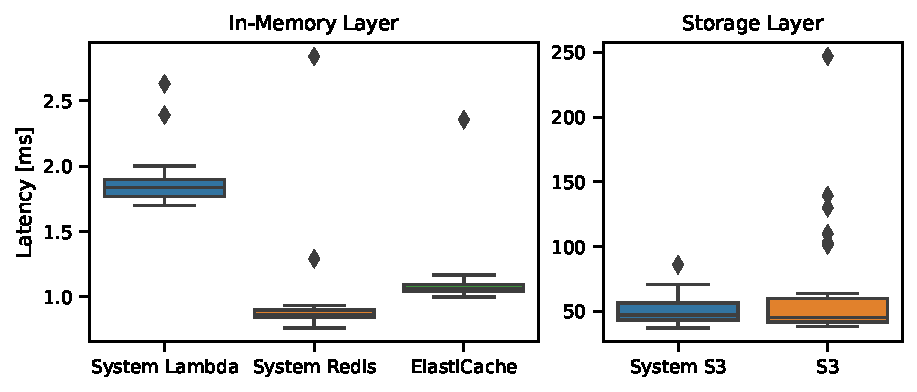
\includegraphics[width=\linewidth]{figures/proxy_latency_100B.pdf}
        \caption{Reverse Proxy latency measurement (100B).}
        \label{fig:proxy_latency_100B}
    \end{subfigure}
    
    \begin{subfigure}{.85\textwidth}
        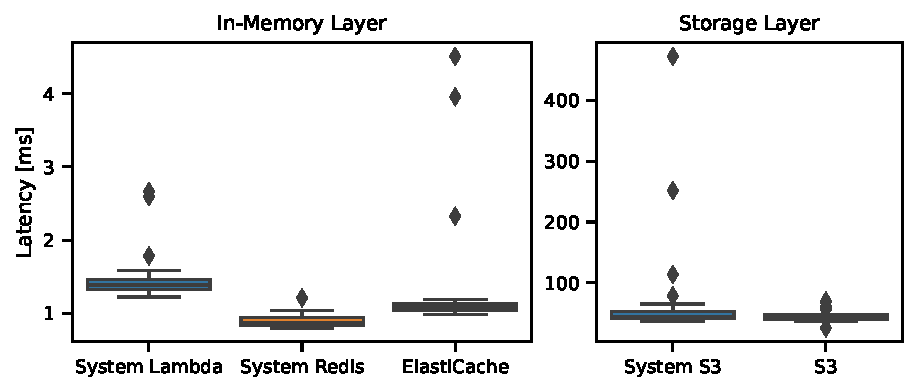
\includegraphics[width=\linewidth]{figures/proxy_latency_1KB.pdf}
        \caption{Reverse Proxy latency measurement (1KB).}
        \label{fig:proxy_latency_1KB}
    \end{subfigure}

    \begin{subfigure}{.85\textwidth}
        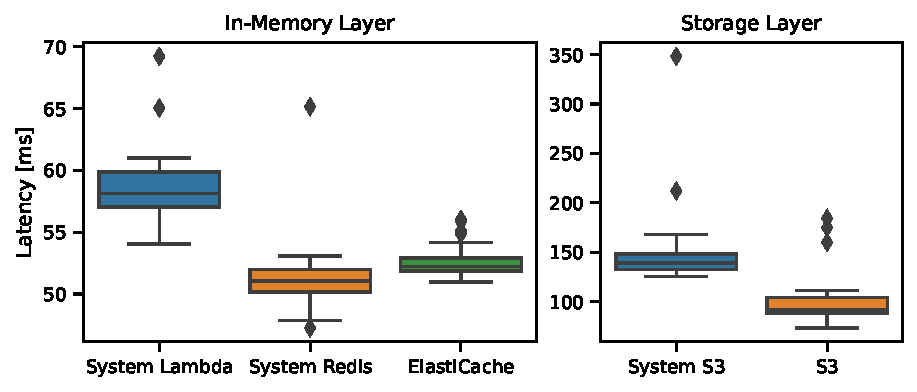
\includegraphics[width=\linewidth]{figures/proxy_latency_1MB.pdf}
        \caption{Reverse Proxy latency measurement (1MB).}
        \label{fig:proxy_latency_1MB}
    \end{subfigure}

    \caption{Measurement of request latency with respect to the reverse proxy. Latency includes the time it takes to process an API request within the AWS infrastructure on the reverse proxy. Each figure contains the measurements for specific object sizes. The left part contains the latency measurements for in-memory layers, while the right part describes the backend memory latency.}
    \label{fig:latency_proxy}
\end{figure}

\begin{figure}[pht!]
    \centering
    \begin{subfigure}{.85\textwidth}
        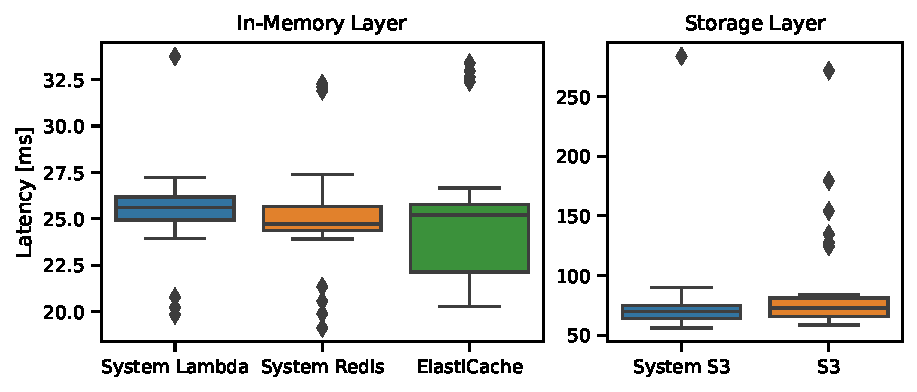
\includegraphics[width=\linewidth]{figures/client_latency_100B.pdf}
        \caption{End-to-end latency measurement (100B).}
        \label{fig:client_latency_100B}
    \end{subfigure}
    
    \begin{subfigure}{.85\textwidth}
        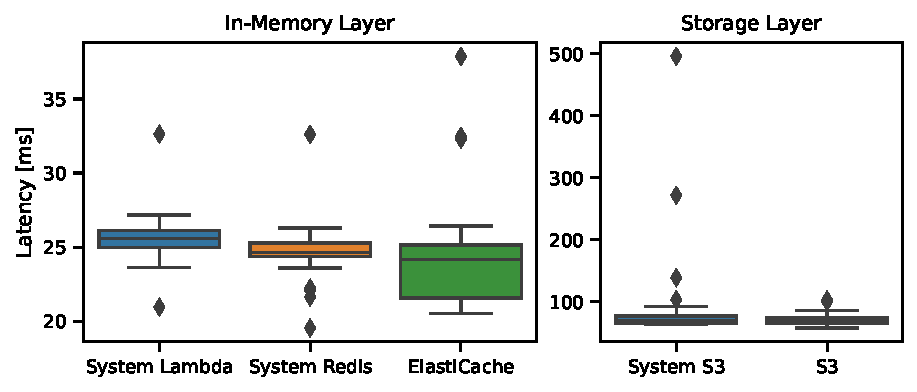
\includegraphics[width=\linewidth]{figures/client_latency_1KB.pdf}
        \caption{End-to-end latency measurement (1KB).}
        \label{fig:client_latency_1KB}
    \end{subfigure}

    \begin{subfigure}{.85\textwidth}
        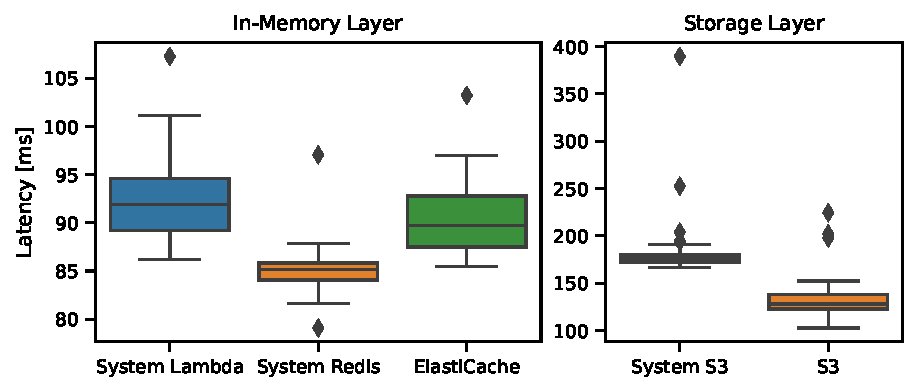
\includegraphics[width=\linewidth]{figures/client_latency_1MB.pdf}
        \caption{End-to-end latency measurement (1MB).}
        \label{fig:client_latency_1MB}
    \end{subfigure}

    \caption{Latency measurement in terms of total end-to-end latency measured on the client in our simulation. Each figure contains the measurements for specific object sizes. The left part contains the latency measurements for in-memory layers, while the right part describes the backend memory latency.}
    \label{fig:latency}
\end{figure}

% Each request is sent 30 times, while we wait 10 seconds between subsequent requests. We manually start the lambda runtime in our system using the control API and make sure that the same function is running for all 30 requests. We ignored the first measurement for the ElastiCache system because the lazy loading technique leads to AWS S3 access on the first request. The object is a simple random text file of a given size, and we repeated the experiment for different object sizes (100B, 1KB, and 1MB).

~\\
% Figure~\ref{fig:client_latency_100B},~\ref{fig:client_latency_1KB}, and~\ref{fig:client_latency_1MB} show the client-side measurements for the different object sizes, while Figure~\ref{fig:proxy_latency_100B},~\ref{fig:proxy_latency_1KB}, and~\ref{fig:proxy_latency_1MB} show the Gin API handler latency measurements from the respective proxy. 
Figure~\ref{fig:latency_proxy} shows the API handler latency measurements from the respective reverse proxy for the different object sizes, while Figure~\ref{fig:latency} shows the client-side end-to-end latency measurements. The results are consistent with the expectation of similar latencies for in-memory systems such as our self-hosted Redis layer, ElastiCache, and even our Lambda function achieves latency of the same order. As expected, the latency measurement for the persistent storage layer is about the same for our system as for a system without in-memory caching. 

~\\
The high latency of Internet traffic is evident when comparing the average latency from an in-memory endpoint for reverse proxy and client measurements. Thus, the average latency for processing an API request on our reverse proxy with the self-hosted Redis endpoint for the 100B object is less than one millisecond, as seen in Figure~\ref{fig:proxy_latency_100B}. In contrast, the average end-to-end latency for the same endpoint and object is about 25 ms, as seen in Figure~\ref{fig:client_latency_100B}. For endpoints with a higher latency on the reverse proxy side, this is no longer as serious in relation to each other. For the 100B object, the additional latency between reverse proxy and end-to-end measurements is approximately 24 ms, regardless of the endpoint. The same order of magnitude remains for the 1KB object. 

~\\
When we look at the reverse proxy measurements for the 1MB object, the storage layer latency increases similar to before between 100B and 1KB. In contrast, the latency increases drastically for each in-memory layer compared to the changes between 100B and 1KB. The reverse proxy copies the received object into the API response, which is a simple copy from the \code{io} package. The duration of the copy is most likely the reason for the increased latency as we approach much bigger objects of one MB. However, we still achieve better end-to-end latency for the in-memory layer than for the storage layer, although the difference is obviously much more significant for smaller objects, which we will focus on in further evaluations. Considering only the reverse proxy latency, the average latency of the in-memory layer for the 100B object is about 1.5 ms, while the memory layer is in the range of 50 ms, resulting in a $33.3\times$ faster in-memory caching retrieval with respect to the reverse proxy latency. Comparing the end-to-end latency, only about $3\times$ faster retrieval is achieved due to the additional latency of the Internet traffic.

\paragraph{Summary.} Both in-memory caching layers in our system achieve latency measurements on the same order of magnitude as ElastiCache. The slower layer S3 results in higher latency, which translates into a $33x$ speedup in terms of reverse proxy latency and a $3\times$ speedup for end-to-end latency due to the significant weight of additional Internet traffic latency. 

\section{Simulations}
\label{subsec:performance_evaluation}
With a better understanding of the latency measurements, we present the simulation results of our system with respect to the different traces used for the simulation. We start by testing our system on a trace modeling the same inter-arrival times of the requests as in the publicly available web server log described in Section~\ref{subsec:simulation_environment}. The extracted queries are for the most frequently queried object over the entire dataset, which includes the logs for one day. The duration of our simulation is one hour and includes all queries from the log for the object within the first hour. We assume the system administrator knows the average rate of requests per minute from the past, which is used for our system configurator. For this specific trace, it is about three requests per minute. For the sensitivity input, we run the simulation for three different values: two, three, and four.
\begin{figure}[t]
    \begin{center}
        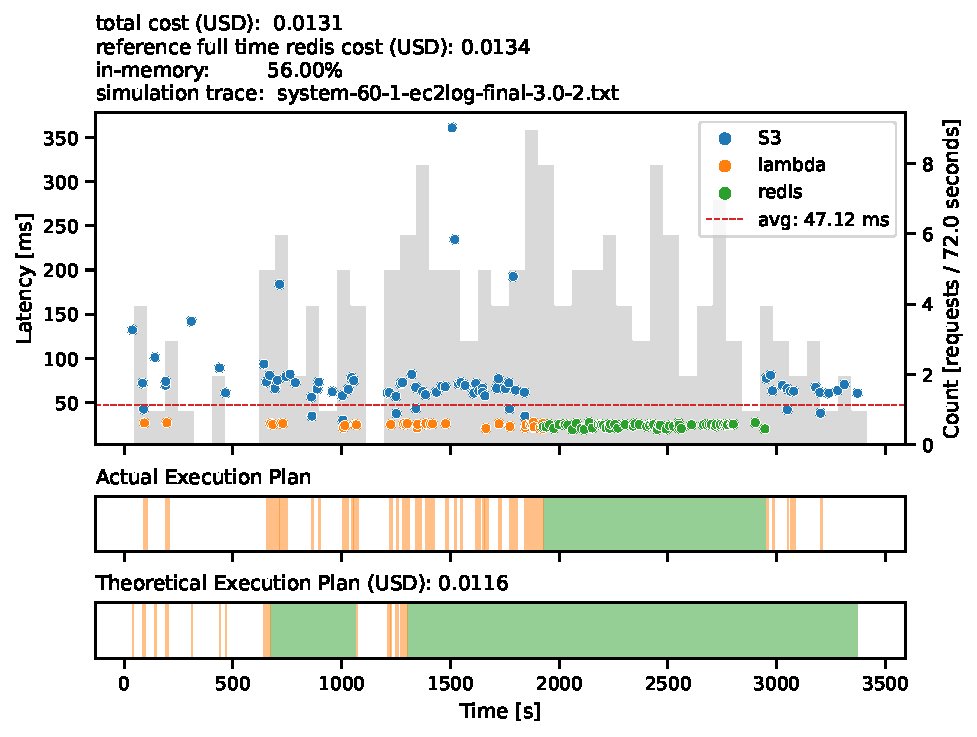
\includegraphics[width=0.8\textwidth]{figures/system-60-1-ec2log-final-3.0-2.pdf}
        \caption{Trace simulation on our system using the system configurator input (rate 3, sensitivity~2).}
        \label{fig:ec2log_3_2}
    \end{center}
\end{figure}

\paragraph{Figure Description.}
First, we provide an overview of the information presented in the simulation Figures such as Figure~\ref{fig:ec2log_3_2}. The x-axis represents the time during the simulation, while the y-axis represents the end-to-end latency measured on the client for each request. Each request is represented individually in the color of the particular endpoint that served the request. The bar chart in the background illustrates the workload distribution with the corresponding bucket size and requests per bucket indicated on the second y-axis on the right. The second subplot is a visualization of the currently active caching layer during the simulation, while the subplot below it visualizes the decision of our offline endpoint scheduler.

\begin{figure}[t]
    \begin{center}
        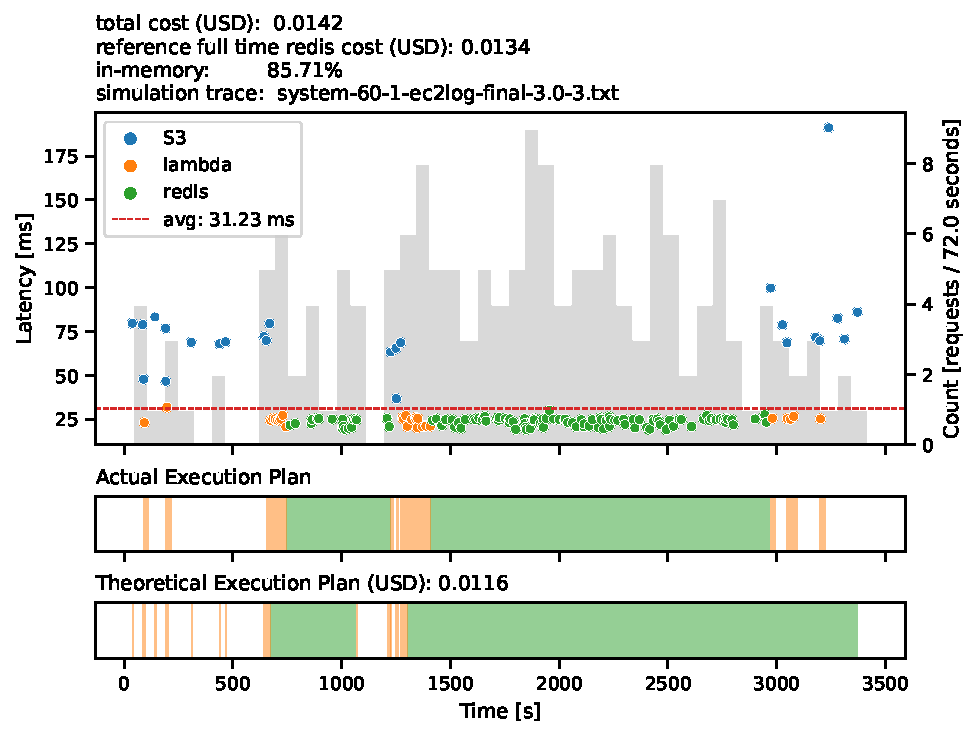
\includegraphics[width=0.8\textwidth]{figures/system-60-1-ec2log-final-3.0-3.pdf}
        \caption{Trace simulation on our system using the system configurator input (rate 3, sensitivity~3).}
        \label{fig:ec2log_3_3}
    \end{center}
\end{figure}

\begin{figure}[t]
    \begin{center}
        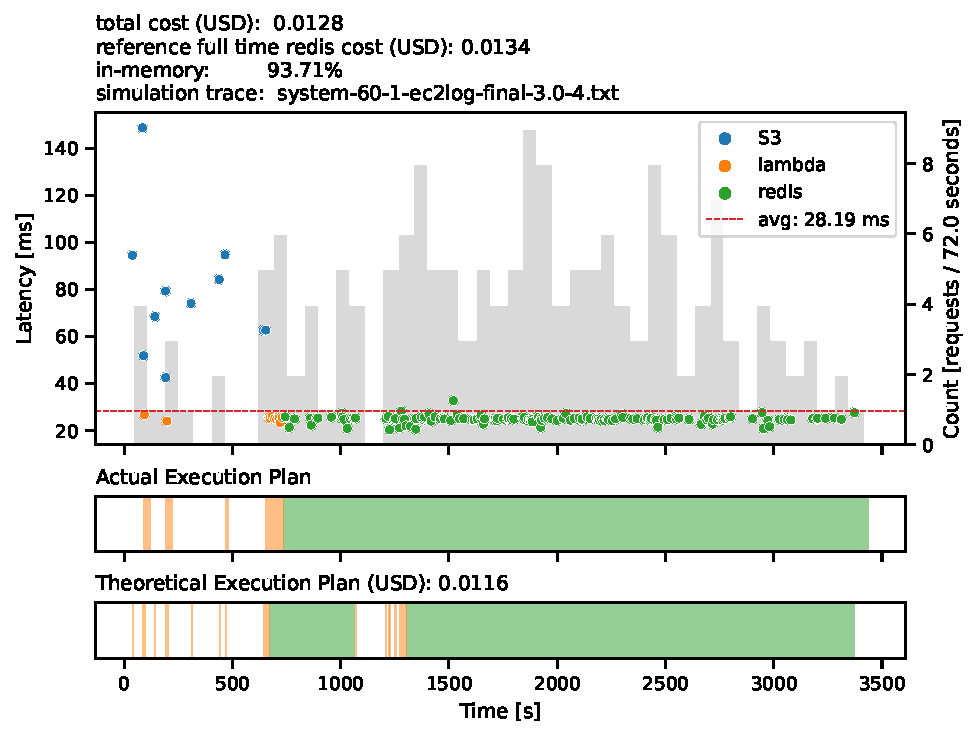
\includegraphics[width=0.8\textwidth]{figures/system-60-1-ec2log-final-3.0-4.pdf}
        \caption{Trace simulation on our system using the system configurator input (rate 3, sensitivity~4).}
        \label{fig:ec2log_3_4}
    \end{center}
\end{figure}

\paragraph{Sensitivity Value.}
The first obvious observation is the strong dependency of system parameters and the resulting endpoint decision-making process as shown in Figure~\ref{fig:ec2log_3_2},~\ref{fig:ec2log_3_3}, and~\ref{fig:ec2log_3_4}. While the rate remains the same in these simulation results, only varying the sensitivity value results in a completely different system at first glance. During the development, we started with fixed system parameters. The first few experiments clearly showed the need for a more dynamically configurable system, which led to the integration of the system configurator. As we increase the sensitivity, we achieve a higher in-memory percentage as expected. So for sensitivity two, only 56\% of the requests are served by either our Lambda runtime or the Redis layer, for sensitivity three we achieve 85.71\%, and for four we even reach 93.71\%. 

~\\
Initially, one would think the higher the sensitivity value, the higher the cost, which is the case for the first two. However, the highest sensitivity value in our experiments is also the experiment with the lowest cost. The reason for this is the more expensive serverless layer compared to the self-hosted Redis, which is used less often than the higher the sensitivity value, as one can easily see in the actual execution plan in the Figures~\ref{fig:ec2log_3_2} to~\ref{fig:ec2log_3_4}. The simulation using a sensitivity value of four achieves an in-memory percentage of 93.71\% and is even cheaper than an always running self-hosted Redis instance of the same type used in our system, but keep in mind that this instance would reach 100\%. 

\paragraph{Offline Endpoint Scheduler.}
When we look at the theoretical execution plan obtained by our offline endpoint scheduler, it is not surprising that the algorithm with the trace known in advance would achieve 100\% in-memory percentage at a lower cost than our system. A more detailed analysis of our endpoint scheduler is presented in the next section. 

\paragraph{Comparison Systems.}
Figure~\ref{fig:comparison_systems} shows the results of the same simulation for the two comparison systems using only S3 and ElastiCache, with lazy loading resulting in S3 access for the first request in ElastiCache. As already explained in the previous section, the end-to-end latencies for the in-memory layer and the storage layer are in the same order of magnitude. ElastiCache achieves an average end-to-end latency of 24.03 ms. Our system with sensitivity 4 achieves a comparable average of 28.19 ms, but as soon as the sensitivity decreases, the average end-to-end latency increases due to the increased number of S3 accesses. A system without in-memory caching as in Figure~\ref{fig:ec2log_s3} obviously achieves the lowest cost, while the price difference for ElastiCache compared to a self-hosted Redis instance is also no surprise but simply a reflection of the price difference of the instance type based on the fully managed service.

% The trace includes 174 requests during the one-hour simulation. So we are nowhere near the point where self-hosted Redis can be cheaper than the cost of S3 requests, as discussed in section~\ref{subsec:comparison_systems}.

\begin{figure}[t]
    \centering
    \begin{subfigure}{.78\textwidth}
        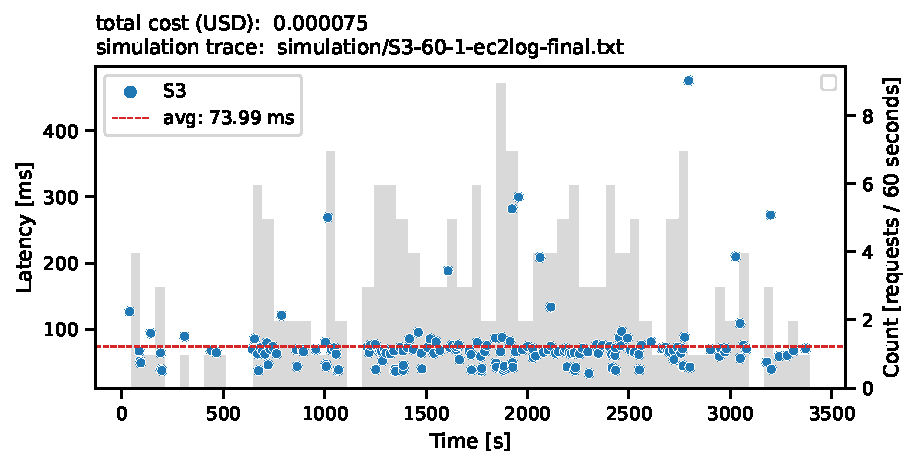
\includegraphics[width=\linewidth]{figures/S3-60-1-ec2log-final.pdf}
        \caption{Simulation on AWS S3 only.}
        \label{fig:ec2log_s3}
    \end{subfigure}
    \begin{subfigure}{.78\textwidth}
        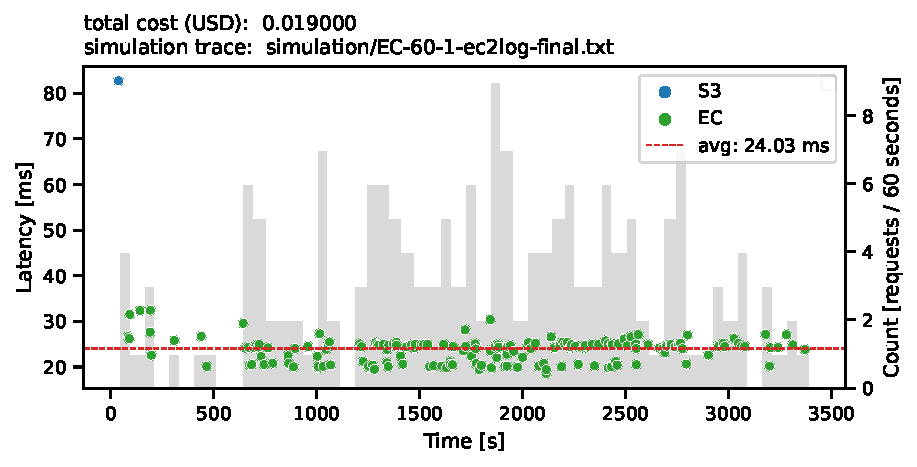
\includegraphics[width=\linewidth]{figures/EC-60-1-ec2log-final.pdf}
        \caption{Simulation on AWS ElastiCache (EC in the figure).}
        \label{fig:ec2log_ec}
    \end{subfigure}
    \caption{Results of the one-hour simulation based on the web server log for the two comparison systems.}
    \label{fig:comparison_systems}
\end{figure}

\paragraph{Varying Workload.}
In order to run our simulation with different traces, we add the method described in Section~\ref{subsec:simulation_environment} to generate traces using a Poisson process. The previous trace does not exactly correspond to a Poisson process, but it also contains an approximately constant average rate of requests. Therefore, we use this method to examine the results for different Poisson process parameters and explore the usability of our system. From the beginning, the goal of our system was to explore the possibilities of integrating the serverless platform as a caching layer into a Redis-based system. The goal was not to design a system that could handle every possible workload, as the design of our system stops making sense once the average request rate is high enough since a constantly running Redis instance will always beat our system in terms of cost at that point. At the same time, a reactive system is useless for workloads with a low average number of requests. More precisely, the advantage of a more expensive and faster reacting serverless layer is not helpful. The simulation results for the Poisson process-based traces in Figures~\ref{fig:poisson_3_23} to~\ref{fig:poisson_4_45} help to understand the design limitations of our system, which we discuss in more detail in the next section with a closer look at our endpoint scheduler. Nevertheless, these results help us understand the design of our system and the use cases where we can actually benefit from a reactive in-memory caching design, as described in Section~\ref{subsec:peak_workload}.

\begin{figure}[pht!]
    \centering
    \begin{subfigure}{.8\textwidth}
        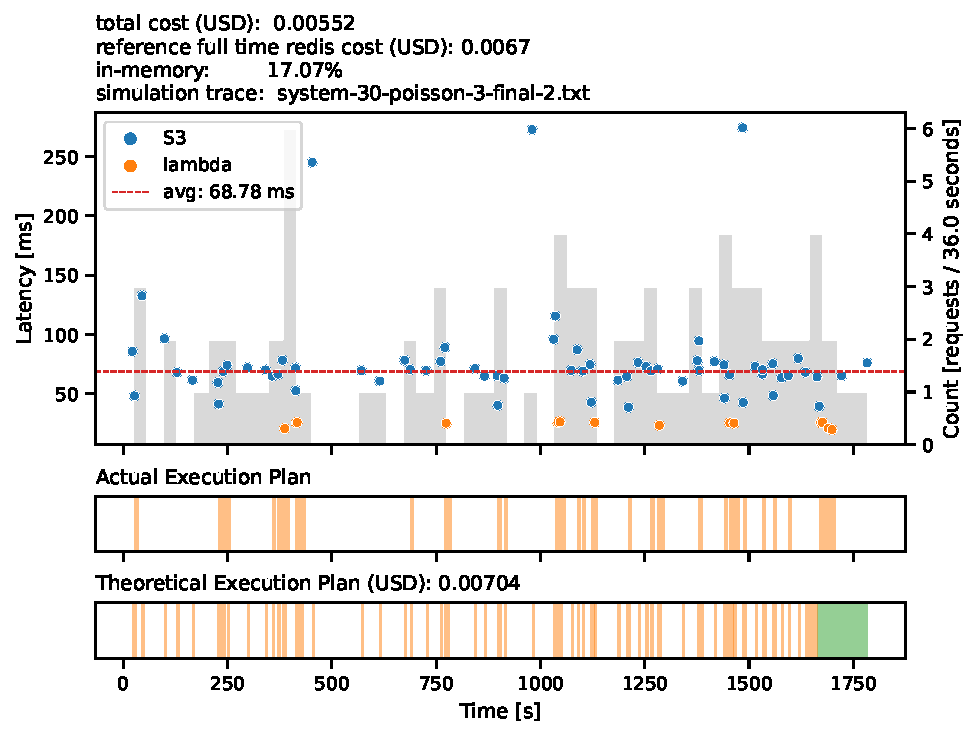
\includegraphics[width=\linewidth]{figures/system-30-poisson-3-final-2.pdf}
        \caption{System configurator used a sensitivity value of 2.}
        \label{fig:poisson_3_2}
    \end{subfigure}
    \begin{subfigure}{.8\textwidth}
        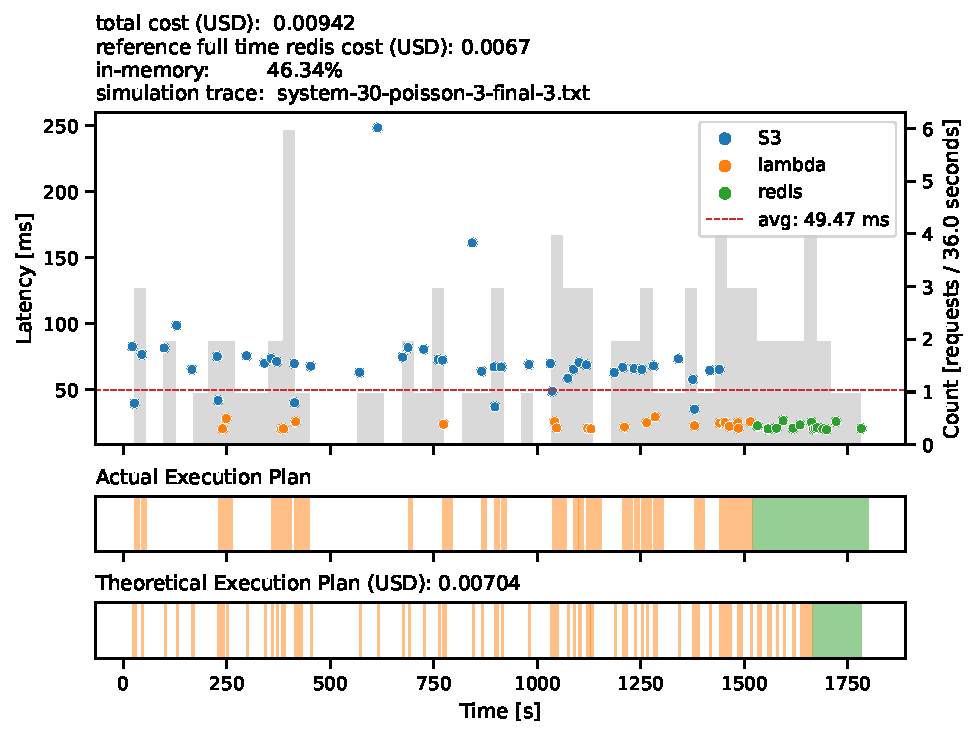
\includegraphics[width=\linewidth]{figures/system-30-poisson-3-final-3.pdf}
        \caption{System configurator used a sensitivity value of 3.}
        \label{fig:poisson_3_3}
    \end{subfigure}
    \caption{Simulations on our system using the rate 3 for the system configurator as the workload is derived as a Poisson process with rate 3. Results for sensitivity values 2 and 3.}
    \label{fig:poisson_3_23}
\end{figure}

\begin{figure}[pht!]
    \centering
    \begin{subfigure}{.8\textwidth}
        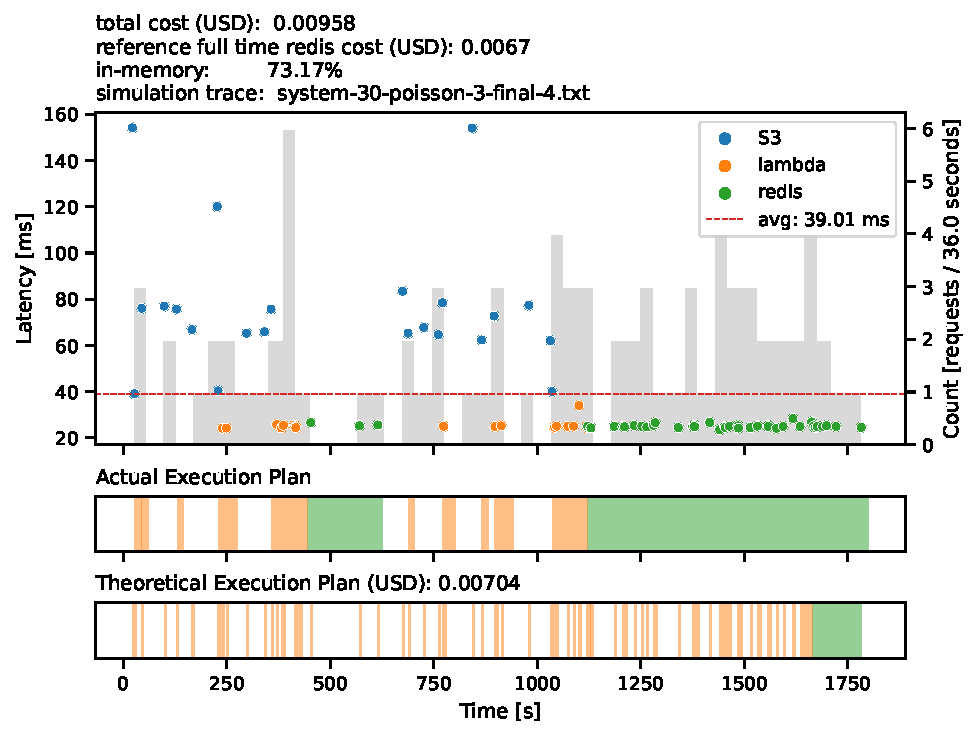
\includegraphics[width=\linewidth]{figures/system-30-poisson-3-final-4.pdf}
        \caption{System configurator used a sensitivity value of 4.}
        \label{fig:poisson_3_4}
    \end{subfigure}
    \begin{subfigure}{.8\textwidth}
        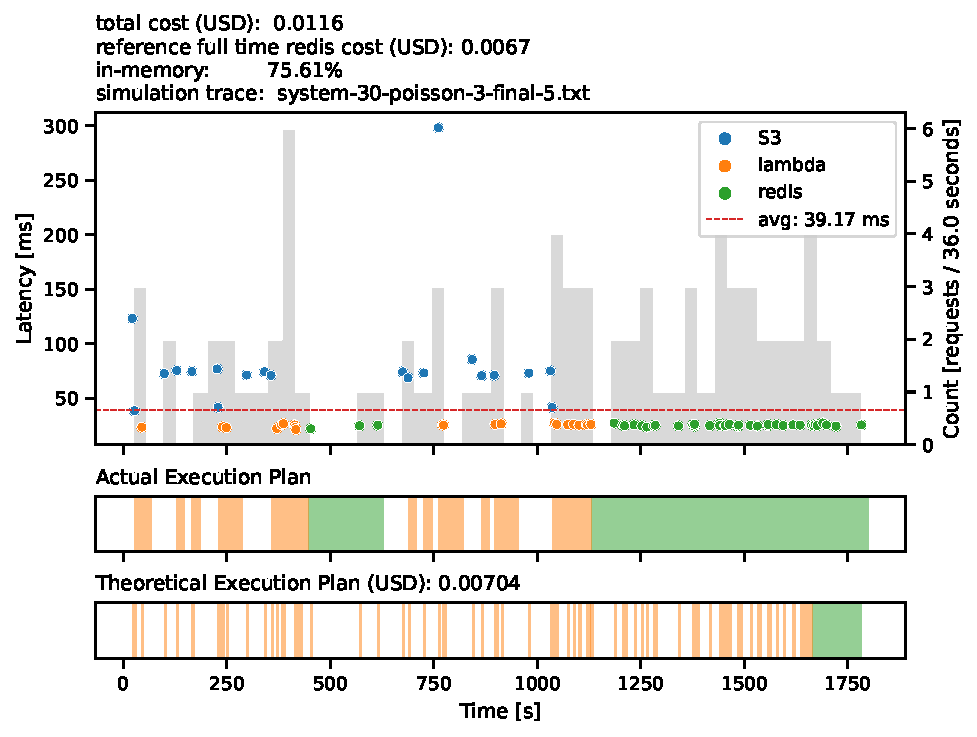
\includegraphics[width=\linewidth]{figures/system-30-poisson-3-final-5.pdf}
        \caption{System configurator used a sensitivity value of 5.}
        \label{fig:poisson_3_5}
    \end{subfigure}
    \caption{Simulations on our system using the rate 3 for the system configurator as the workload is derived as a Poisson process with rate 3. Results for sensitivity values 4 and 5.}
    \label{fig:poisson_3_45}
\end{figure}

\begin{figure}[pht!]
    \centering
    \begin{subfigure}{.8\textwidth}
        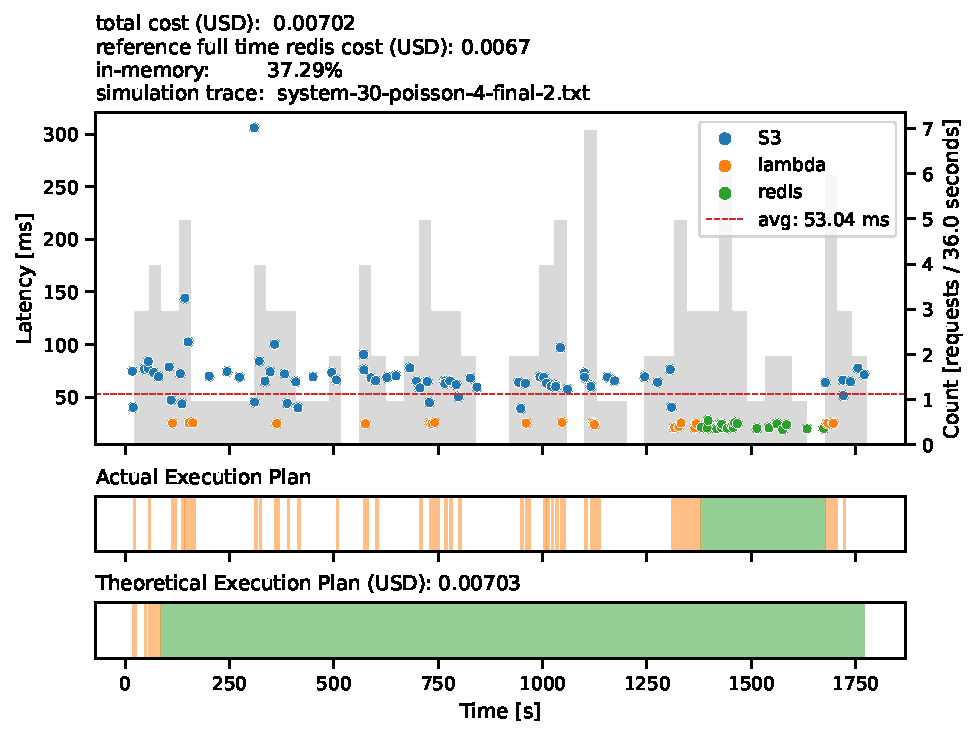
\includegraphics[width=\linewidth]{figures/system-30-poisson-4-final-2.pdf}
        \caption{System configurator used a sensitivity value of 2.}
        \label{fig:poisson_4_2}
    \end{subfigure}
    \begin{subfigure}{.8\textwidth}
        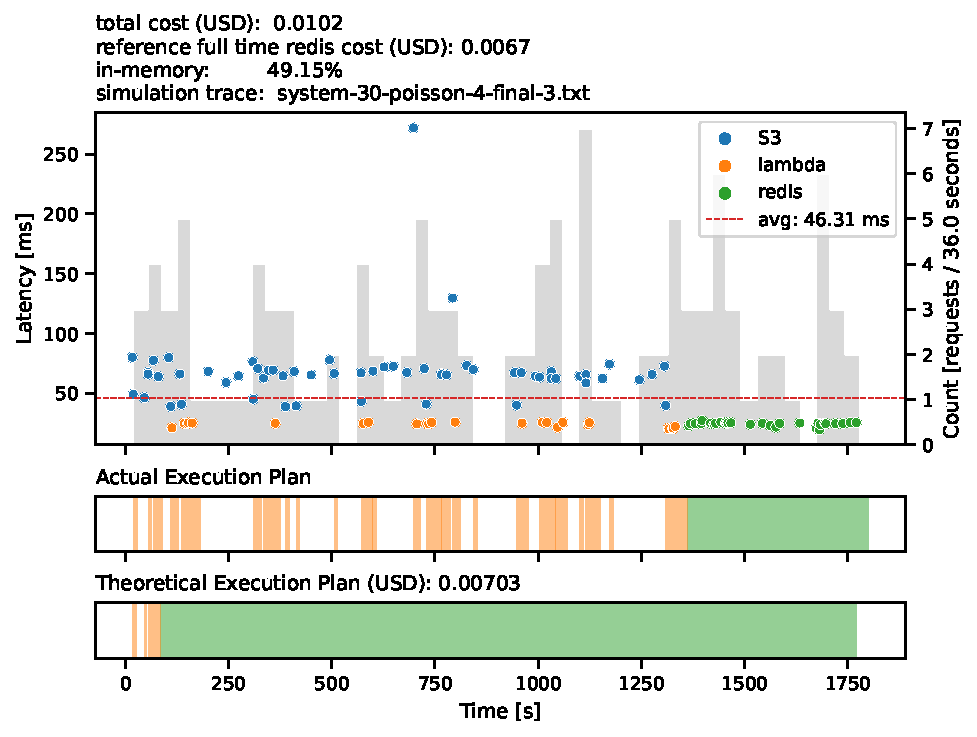
\includegraphics[width=\linewidth]{figures/system-30-poisson-4-final-3.pdf}
        \caption{System configurator used a sensitivity value of 3.}
        \label{fig:poisson_4_3}
    \end{subfigure}
    \caption{Simulations on our system using the rate 4 for the system configurator as the workload is derived as a Poisson process with rate 4. Results for sensitivity values 2 and 3.}
    \label{fig:poisson_4_23}
\end{figure}

\begin{figure}[pht!]
    \centering
    \begin{subfigure}{.8\textwidth}
        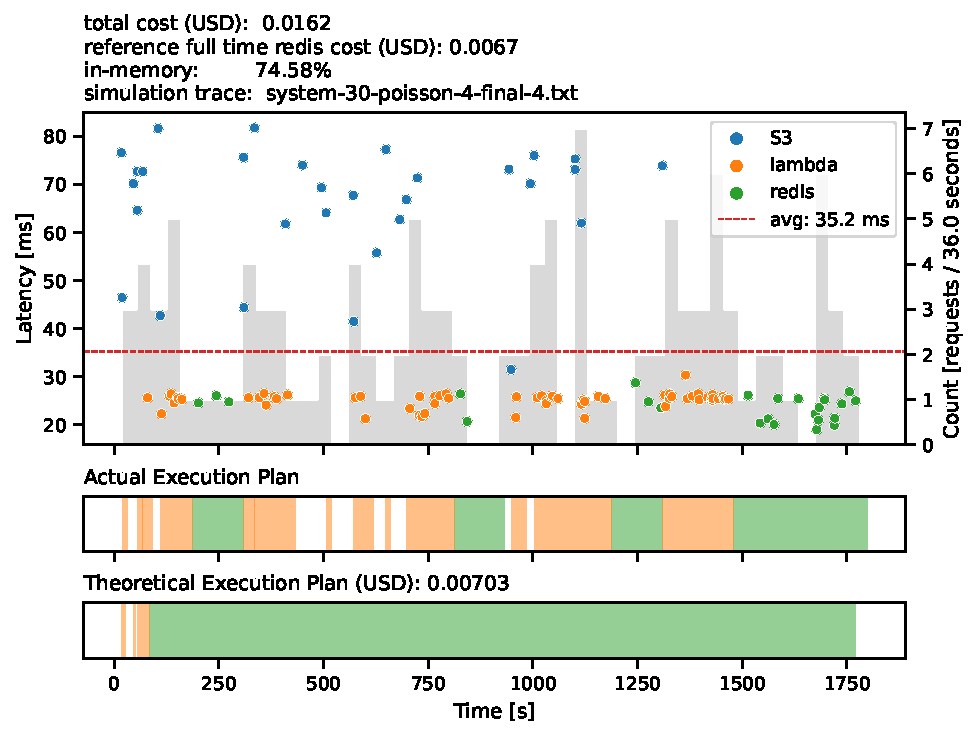
\includegraphics[width=\linewidth]{figures/system-30-poisson-4-final-4.pdf}
        \caption{System configurator used a sensitivity value of 4.}
        \label{fig:poisson_4_4}
    \end{subfigure}
    \begin{subfigure}{.8\textwidth}
        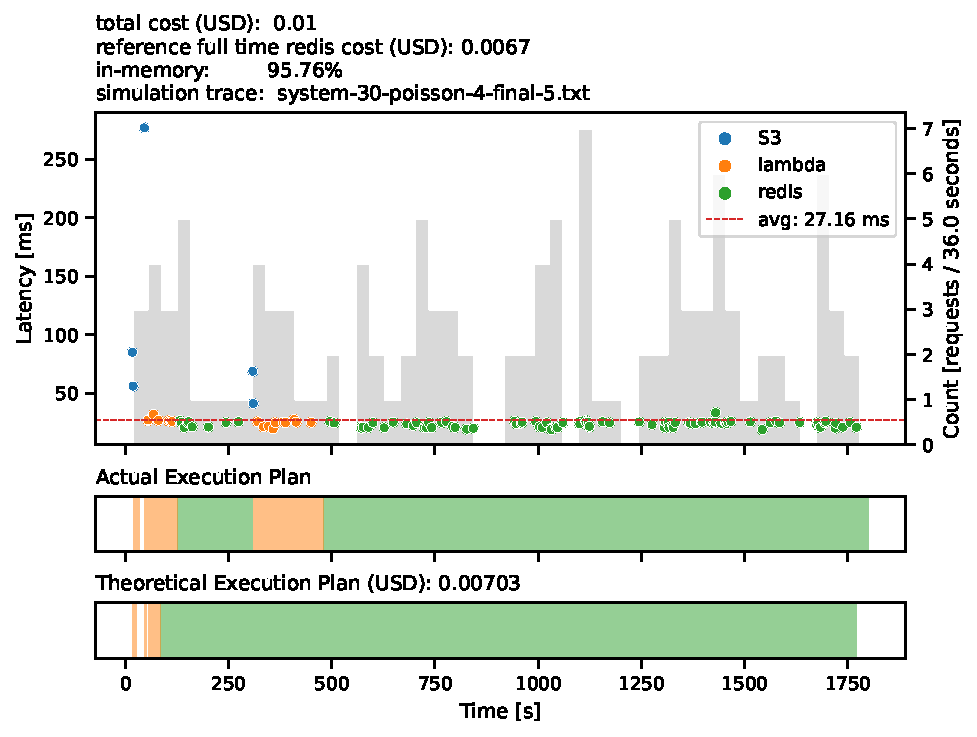
\includegraphics[width=\linewidth]{figures/system-30-poisson-4-final-5.pdf}
        \caption{System configurator used a sensitivity value of 5.}
        \label{fig:poisson_4_5}
    \end{subfigure}
    \caption{Simulations on our system using the rate 4 for the system configurator as the workload is derived as a Poisson process with rate 4. Results for sensitivity values 4 and 5.}
    \label{fig:poisson_4_45}
\end{figure}

\paragraph{Summary.}
We use the simulations to explore the usability of our system. The close dependence between the system parameters and the workload in terms of in-memory percentage and cost is quickly apparent. The results show some clear limitations of our system for use as a cost-effective caching system for general workloads. For example, either response time does not matter if the frequency of requests is too low, or a reactive design is meaningless if caching is desired all the time. The results in this section form the basis for discussing our endpoint scheduler in the next section.

\section{Endpoint Scheduler}
\label{sec:endpoint_scheduler}
% analyze the behaviour and performance of our endpoint scheduler
% explain their impact on the system with trace examples and actual simulations.
% conclusion should be that the design our system target to enhance the speedup to make in-memory caching available -> so unexpected peak workloads are of interest
The previous section briefly introduced the strong dependence of the system parameters and the resulting endpoint decision process on our endpoint scheduler. We use the simulations presented to shed more light on this dependence. For the purposes of this discussion, the system parameters for the specific inputs to the system configurator are shown in Table~\ref{tab:system_configurator}.

\paragraph{System Parameters in Action.}
The independent parameters \emph{lambdaWindowElements} and \emph{redisThreshold} determine the number of requests required to be resolved by the previous layer within specific time duration to transition to the new layer and therefore to a new state as shown in Figure~\ref{fig:endpoint_scheduler}. The mentioned time duration is the part for which our system configurator derives different values depending on the input. For example, for \emph{lambdaWindowElements}, the requests must be received within the time window specified by the \emph{lambdaThreshold}, while \emph{redisThreshold} is linked to the \emph{TICK} duration, which determines how long the Lambda runtime will run. The last system parameter \emph{redisUtilization} specifies the time in which the last five requests for our Redis layer must have arrived; otherwise, the Redis layer is stopped. Therefore, this parameter represents the tolerance of whether we keep our Redis layer running. Thus, depending on these parameters, our endpoint scheduler's trade-off in maintaining in-memory caching layers versus cost savings is clearly evident.

~\\
So as we increase the \emph{TICK} duration, the possibility of two subsequent requests being forwarded to the same Lambda runtime invocation increases. Since the \emph{TICK} duration is also used to extend the timeout functionality on our Lambda runtime, a larger \emph{TICK} duration also increases the probability of reaching the \emph{redisThreshold} and thus switching to the Redis-based part of our system. The downside of increasing the \emph{TICK} duration is the increased cost of the longer-running Lambda layer. The \emph{lambdaThreshold} defines the granularity at which our system actually starts any state transitions, so if we never receive two subsequent requests within this duration, our system is stuck in the \textsc{S3} state and will never make use of the in-memory caching layers. This duration should help anticipate the arrival of multiple requests in the future. At this point, we want to deploy in-memory caching while not being too reactive and starting the Lambda layer every time a single request arrives. With a general understanding of our system parameters, we now look at the simulation results with a focus on the endpoint scheduler.

\begin{table*}[t]
    \centering
    \ra{1.1}
        \begin{tabular}{ @ {} r r c r r r @ {}}
        \toprule
        \multicolumn{2}{c}{Configurator Input} & \phantom{abc} & \multicolumn{3}{c}{System Parameters} \\
        \cmidrule{1-2} \cmidrule{4-6}
        rate  & sensitivity && \emph{TICK} & \emph{lambdaThreshold} & \emph{redisUtilization} \\
        \midrule
        3 & 2 && 8s  & 16s & 2m20s \\
        3 & 3 && 12s  & 24s & 2m40s \\
        3 & 4 && 16s  & 32s & 3m00s \\
        4 & 2 && 6s  & 12s & 1m45s \\
        4 & 3 && 9s  & 18s & 2m00s \\
        4 & 4 && 12s & 24s & 2m15s \\
        6 & 2 && 4s  & 8s & 1m10s \\
        6 & 3 && 6s & 12s & 1m20s \\
        6 & 4 && 8s & 16s & 1m30s \\
        9 & 4 && 5s & 10s & 1m00s \\
        \bottomrule
        \end{tabular}
    \caption{Comparison of different system parameters depending on the system configurator input. Two system parameters are chosen independently of the input and are therefore omitted from the table. The \emph{lambdaWindowElements} is set to 2 and the redisThreshold to 4.}
    \label{tab:system_configurator}
\end{table*}

\paragraph{Simulation Analysis.}
The results for the web server log trace experiments, which all used a rate of 3 for the system configuration, vary widely. This is due to the changing system parameters caused by the varying sensitivity value. Figure~\ref{fig:ec2log_3_2} shows that the duration of \emph{lambdaThreshold} is low enough to trigger the transition to Lambda multiple times. However, the duration of \emph{TICK} appears to be too low to capture many requests and also results in only a single transition to the Redis-based system. So our system often starts the Lambda layer without serving many requests from it, which causes the higher total costs compared to the simulation using sensitivity three in Figure~\ref{fig:ec2log_3_3}. A closer look at the cost composition clearly confirms our assumption. The total billed duration for the Lambda layer is about 394 seconds compared to the 556 seconds for the lower sensitivity value. Thus, for sensitivity value two, \$0.00929 of total \$0.0131 is spent on the runtime duration for the serverless layer alone, while for sensitivity value three, only \$0.0066 of \$0.0142 is spent. The higher total cost for the higher sensitivity value is thus caused by the much longer runtime of the less expensive Redis layer, which also explains the much higher in-memory percentage. The influence of \emph{redisUtilization} becomes clear when we compare Figure~\ref{fig:ec2log_3_3} and Figure~\ref{fig:ec2log_3_4}. In the beginning, they are quite similar, but the lower \emph{redisUtilization} causes the Redis instance to be shut down, while a higher sensitivity value keeps the Redis instance alive in the same scenario, resulting in a higher in-memory percentage and lower overall cost by avoiding the more expensive Lambda runtime which is used almost immediately after the instance is shut down to transition back to the Redis state.

\paragraph{Endpoint Scheduler Limitations.}
We experiment with the Poisson process-based traces to evaluate the endpoint scheduler for multiple traces and thus different workload characteristics. Our expectation regarding the limited usability of our system with a more or less constant request rate modeled as a Poisson process was quickly confirmed. The results in terms of cost efficiency were poor compared to the web server log trace. The theoretical execution plan provides an interesting insight for this discussion. Once the rate is too low, our offline endpoint scheduler basically avoids using the Redis-based layer and uses only the serverless layer, as shown for the Poisson process trace for rate three in Figure~\ref{fig:poisson_3_23}. The result for our offline endpoint scheduler is exactly the opposite if we increase the Poisson process rate to four: it keeps the Redis layer all the time while using the Lambda layer only at the beginning, as shown in Figure~\ref{fig:poisson_4_23}. Increasing the sensitivity does lead to a higher percentage of in-memory with the consequence of higher costs. However, due to the constant request rate, we never really benefit from the reactive design of our system. 

~\\
Compared to the web server log, where our system saves costs in the first ten minutes because almost no requests arrive, and thus no in-memory layer is urgently needed. Thus, if we reconsider our interpretation of the similarity of the web server log to a Poisson process, we see the significance of the two peaks. The simulation in Figure~\ref{fig:ec2log_3_3} marks these peaks during the periods when our system is running the Redis layer. The break between the peaks is very short, so we can save costs by running the Redis layer between these peaks, as is the case with the higher sensitivity value. In summary, the design of our system targets peak workloads where we can actually benefit from the responsiveness and design of our system. Attempting to build a general caching system with our system configurator is already severely compromised by design and does not appear to be goal-oriented. For this reason, we are focusing for now on workload peaks where the design of our system is critical.

\paragraph{Summary.}
A closer look at the endpoint scheduler and its system parameters in the context of the simulations helps to understand the tight dependency mentioned in the previous section. The current design of our system is understandably not for general workloads, which is nicely emphasized by the offline endpoint scheduler for the Poisson process traces. The reactive design of our system is clearly designed for bursty workloads, which will be discussed in the next section. 

\section{Bursty Workload}
\label{subsec:peak_workload}

\begin{figure}[t]
    \begin{center}
        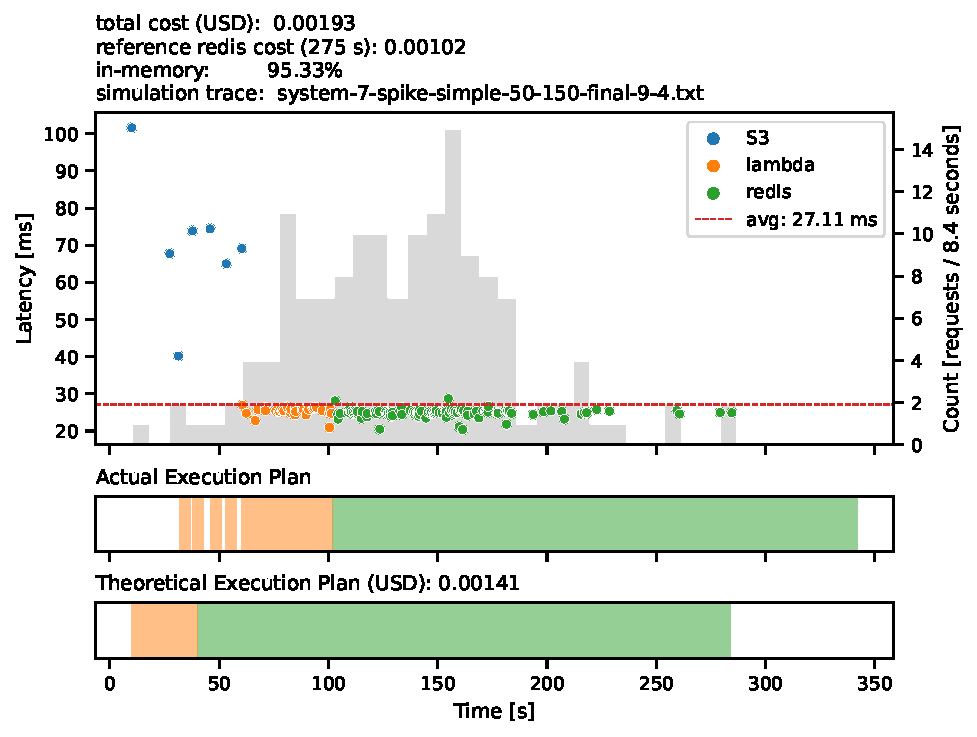
\includegraphics[width=0.8\textwidth]{figures/system-7-spike-simple-50-150-final-9-4.pdf}
        \caption{The arrival times for 150 requests were taken from a normal distribution with a standard deviation of 50 seconds to simulate a peak load on our system.}
        \label{fig:spike_1}
    \end{center}
\end{figure}

\begin{figure}[t]
    \begin{center}
        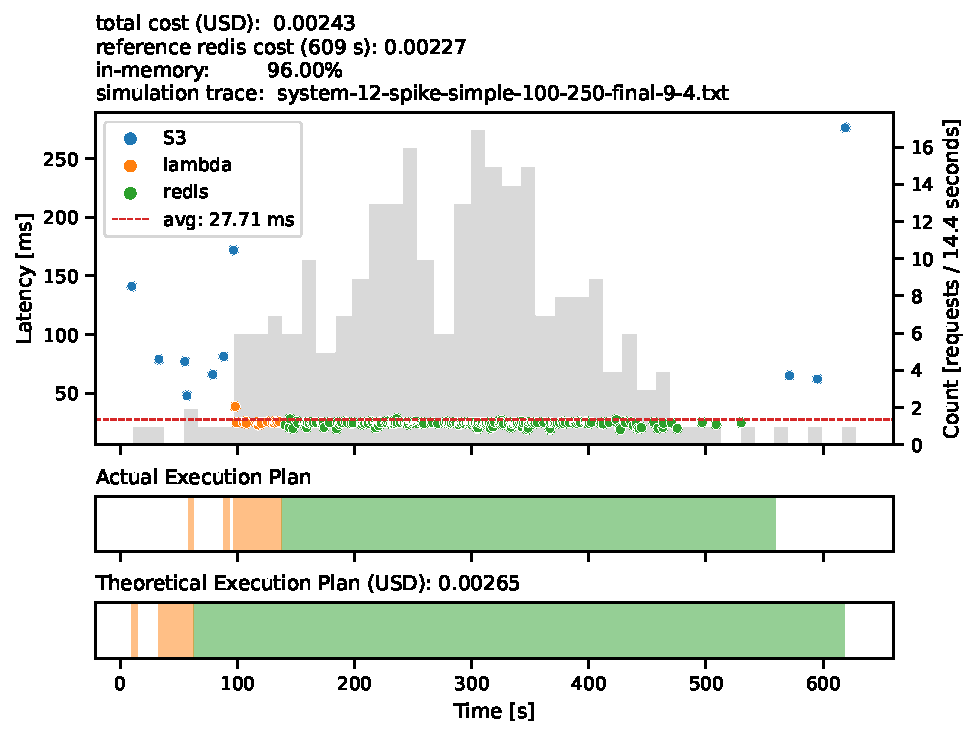
\includegraphics[width=0.8\textwidth]{figures/system-12-spike-simple-100-250-final-9-4.pdf}
        \caption{The arrival times for 250 requests were taken from a normal distribution with a standard deviation of 100 seconds to simulate a peak load on our system.}
        \label{fig:spike_2}
    \end{center}
\end{figure}
When focusing on burst workloads, we can safely assume that at some point, enough requests are received to trigger the state transition on our endpoint scheduler. Therefore, the system parameters become drastically less important. Nevertheless, the system parameters still play an important role depending on the tail distribution of the peak since they indicate how fast our system reacts to an approaching spike and how it behaves when the peak drops. To investigate more on the behavior of our system during spike workloads, we run additional experiments using the \emph{spike-simple} method described in Section~\ref{subsec:simulation_environment}. It uses a normal distribution to model the spike while the simulation duration is limited to the actual samples from the distribution. In the context of these experiments, we assume that the arrival time of the spike is unknown while the rate during the spike is high enough so that a Redis instance is always more cost-effective than Lambda. While we vary the duration of these spikes by taking more samples from a normal distribution with a higher standard deviation, we focus on spikes that last less than one hour. Therefore, comparing our system with ElastiCache is not of much interest due to the billing granularity of node hours. Nevertheless, when we look at the arrival frequency of these spikes at the end, we include ElastiCache again in our discussion. 

\paragraph{Perfect Automation Process.}
Remember the perfect automation process for a self-hosted Redis-based system, described at the end of Section~\ref{subsec:comparison_systems}. The perfect automation process provides a lower bound with respect to cost for a Redis-based system where the instance is exactly running as soon as we receive the first request and shut down after the last request was received. This would require knowing the trace in advance and starting the instance at just the right time so that it does not run too early, which would add some overhead. The baseline provided by this comparison system helps evaluate the cost-effectiveness of our system for these experiments. Thus, the reference costs shown in the charts are no longer a full-time Redis instance but only include the billed duration between the first and the last request.

\begin{figure}[t]
    \begin{center}
        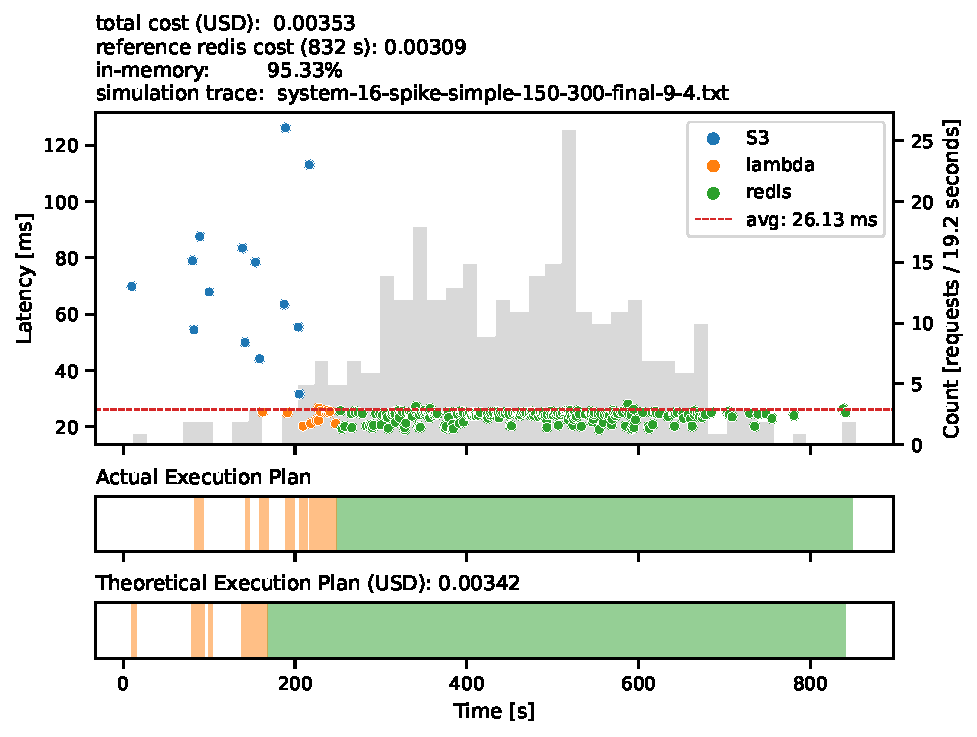
\includegraphics[width=0.8\textwidth]{figures/system-16-spike-simple-150-300-final-9-4.pdf}
        \caption{The arrival times for 300 requests were taken from a normal distribution with a standard deviation of 150 seconds to simulate a peak load on our system.}
        \label{fig:spike_3}
    \end{center}
\end{figure}

\begin{figure}[t]
    \begin{center}
        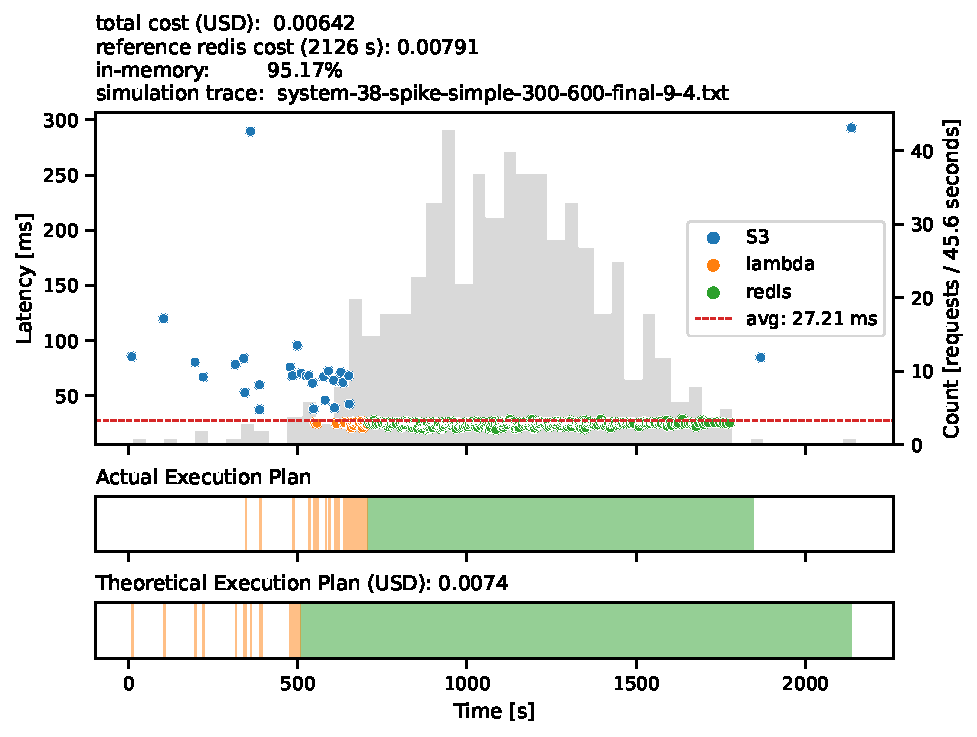
\includegraphics[width=0.8\textwidth]{figures/system-38-spike-simple-300-600-final-9-4.pdf}
        \caption{The arrival times for 600 requests were taken from a normal distribution with a standard deviation of 300 seconds to simulate a peak load on our system.}
        \label{fig:spike_4}
    \end{center}
\end{figure}

\paragraph{Simulation Results.}
First, we present the results for different spike durations where we used the system parameters shown in the last row of Table~\ref{tab:system_configurator}. The way our system configurator is designed is not really intended to optimize the performance of our system with respect to spike workloads. For this reason, we fix the system parameters for these experiments and discuss their effects at the end and consider how they could be improved. 

~\\
We find that we achieve a similar in-memory percentage between 95\% and 96\% for each peak, with a big difference when we compare the actual cost of our system to the Redis-based reference system. Thus, for a short peak as in Figure~\ref{fig:spike_1}, our system is almost twice as expensive, while for the longer-lasting peak as in Figure~\ref{fig:spike_4} we are even cheaper. An important point regarding cost is the usage of the serverless layer, which is a less cost-efficient in-memory caching layer than the self-hosted Redis instance. While the number of calls and the total runtime of our Lambda layer still depends on the actual distribution of requests arriving at our system, their proportional share in the total cost decreases significantly. For the simulation in Figure~\ref{fig:spike_1}, the billed Lambda duration is responsible for 53\% of the total cost, while the percentage is between 33-36\% for the other three experiments. 

~\\
So we can argue that our system is less cost-effective with a short peak duration, but on the other hand, handling a short peak duration with an automation process is even more difficult. So if the automation process only responds by starting the Redis instance as soon as the first request comes in, this could result in several EC2 billing minutes where only a single request is received and no actual peak. When a peak comes in, we miss a large portion of the peak while the automation process starts the instance. The fraction missed by a reactive automation process decreases as the duration of the spike increases, but this leads to another interesting discussion about the tail distribution of the peaks. 

\paragraph{Tail Distribution.}
So while a perfect automation process for self-hosted Redis would achieve 100\% in-memory caching, it runs at the beginning of the peak and continues to run until the last request is received. This results in a total runtime of 2126 seconds for the Redis reference instance in Figure~\ref{fig:spike_4} while the combined runtime of our caching layers totals only 1270 seconds. We thus achieve an in-memory percentage of 95.17\%, while running the in-memory layer only 60\% of the time. 

~\\
This effect is somewhat limited to the shorter peaks by our current system configurator's previously mentioned adjustability limitation. Thus, with the system parameters, we can control our system's responsiveness and set the tolerance threshold for shutting down a running in-memory layer. While the responsiveness is quite satisfying with respect to the experiments, we notice a problem in the current configurator design when handling short peak durations. Recall that our endpoint scheduler reevaluates once a minute if the Redis layer should be kept alive using the \emph{redisUtilization} system parameter. In the case of a short spike duration, the granularity at which we do this check is obviously a big problem, as shown in Figure~\ref{fig:spike_1}. However, the problem we mentioned regarding the system configurator is related to the way we derive the \emph{redisUtilization}. Because for a short spike duration, we want to keep the other system parameters but reduce the \emph{redisUtilization} to react faster when the end of the spike is approaching, which is currently not possible with our system configurator.

\begin{table}[t]
    \centering
    \ra{1.2}
        \begin{tabular}{ @ {} r c r r c r r @ {} }
        \toprule
        \multicolumn{1}{c}{} & \phantom{abc }& \multicolumn{2}{c}{Self-Hosted Redis} & \phantom{abc} & \multicolumn{2}{c}{AWS ElastiCache} \\
        \cmidrule{3-4} \cmidrule{6-7}
        spike duration &&  spikes  & hourly coverage &&  spikes  & hourly coverage \\
        \midrule
        275s && 6 & $45\%$ && 9 &  $68\%$ \\
        609s && 5 & $84\%$ && 7 & $>100\%$ \\
        832s && 3 & $69\%$ && 5 &  $>100\%$ \\
        2126s && 2 & $>100\%$ && 2 & $>100\%$ \\
        \bottomrule
        \end{tabular}
    \caption{For each experiment in this section, we give the maximum number of spikes that can occur during an hour so that our system still results in a lower cost than the two comparison systems. We also calculate the percentage of an hour that the number of spikes could span without overlapping.}
    \label{tab:spikes}
\end{table}

\paragraph{Burst Frequency.}
Comparing our system with respect to a perfect automation process makes sense when focusing on a single peak. However, we can only argue about the theoretical lower bound for the cost point, motivating our system with the difficulty of developing a prediction-based automation process that never results in unnecessarily launched Redis instances and always responds in a timely manner. Turning the discussion back to the systems we already used in the evaluation section, we now consider the given spike distributions and discuss the frequency with which these spikes can occur, keeping our system cheaper than an always running self-hosted Redis instance and ElastiCache. 

~\\
The price per hour for the self-hosted Redis instance (\code{t2.micro}) is \$0.0134, while the ElastiCache instance (\code{cache.t2.micro}) costs \$0.019 per hour. For simplicity, we assume that the spikes repeat without overlapping each other. Furthermore, we assume that the arrival times are still random and thus unpredictable to counter the automation argument with respect to the self-hosted Redis automation process. Table~\ref{tab:spikes} shows the number of spikes within an hour for which our system costs less compared to the two comparison systems, as well as the percentage of an hour covered by the duration of the given number of spikes arriving during that hour. Using a reactive in-memory caching management system can clearly help in such situations, even if we never achieve 100\% in-memory caching. If this is not an urgent requirement and the goal is to save some costs without worrying about an automation process under the assumption that predicting the workload is rather difficult, the reactive design of our system offers a promising solution.

\paragraph{Summary.}
When we consider burst workloads, we consistently achieve a high in-memory percentage of about 95\%. The cost-efficiency of our system compared to perfectly scheduled self-hosted Redis strongly depends on the duration of the peak for two reasons. One reason is the less cost-effective serverless layer, which loses weight as the duration increases. The other point is critical for short peaks because the current implementation limits the elasticity of our system in terms of shutting down the Redis instance after the peak. Nevertheless, our system achieves remarkable results for burst workloads. We achieve costs close to those of a self-hosted Redis instance running exactly for the workload duration with an in-memory percentage of 95\%. We even achieve this percentage for long-tail distributions, but at a lower cost than self-hosted Redis. So, considering how difficult it is to start self-hosted Redis in a cost-effective way for these bursts with unknown arrival times, this really shows the potential of a reactive design using serverless computing.

% motivate why the system parameters are not the focus of this evaluation (system configurator designed to handle the "tolerance" of our system, wile we now want a reasonable TICK and lambdaThreshold without increasing the redisUtilization which leads to poor performance for our system for the end of the spike)

% simple spike evaluations for different normal distributions
% -> just a single system parameter configuration or multiples?

% conclusion should be that the design our system target to enhance the speedup to make in-memory caching available -> so unexpected peak workloads are of interest
% analyze at what frequency of a specific peak are we cheaper than redis all the time with the tradeoff of a few S3 accesses (also compare to ElastiCache?)
% analyze the number of S3 accesses (connected to system configuration and tail distribution of the peak)

\section{Startup Times}
\label{subsec:startup_times}
% evaluation of the startup times
% lambda (different object sizes, cold vs warm startup)
% self-hosted redis (different object sizes, multiple objects?)
Focusing on a reactive system design leads to the question of how fast our system provisions the in-memory caching layers. This section presents the startup times of the self-hosted Redis instance and the time it takes for the serverless layer to become available in terms of cold and warm starts. 

\paragraph{Experiment Description.}
In the context of these experiments, the reverse proxy logs the time\-stamps of requests received from the client that will trigger a state transition to the \textsc{Lambda} or \textsc{RedisBootup} state on the orchestrator. In addition, the reverse proxy logs the timestamp whenever the \emph{LambdaStart} or \emph{RedisUpdate} message changes the forwarding on the reverse proxy. Thus, the time difference indicates the time needed to react and provide the in-memory caching layer so that the reverse proxy can use it for the subsequent request. In all scenarios, the time also includes the additional message delivery delay to inform the orchestrator about the received request. For self-hosted Redis, the orchestrator must send an additional message once the instance is up and running to inform the reverse proxy about the object served by the Redis endpoint, while Lambda runtime also sends a message to inform about the available endpoint. Self-hosted Redis and cold starts for Lambda need to download the object from S3 additionally. The experiments are performed in the same environment as the other simulations, and each measurement is repeated 30 times for different object sizes.
% though this latency is not really relevant as you can see for different object sizes

\paragraph{Results.}
Figure~\ref{fig:startup} clearly shows the different time dimensions needed until the in-memory caching layer is available to the reverse proxy. Increasing the object size results in a slight increase due to the required download of the object, as shown for the Lambda cold start and the self-hosted Redis instance, although the increase is relatively small compared to the overall latency of the startup process. Warm Lambda startup times do not depend on object size because the object remains available within the reused execution environment. So the time it takes for our self-hosted Redis layer to become available is about 30 seconds, while Lambda takes about 600 ms in the case of a cold start and only about 20 ms in the case of a warm start. In terms of the reactive design of our system, the Redis layer takes about $50$--$1500\times$ longer to become available compared to the serverless layer.

\paragraph{Summary.}
The fast startup times of serverless functions are no surprise and therefore offer a great additional in-memory caching layer for a reactive system. Such a system can greatly benefit burst workloads with unknown arrival times, as a reactive system provides the ability to reduce costs without sacrificing a large portion of the load by missing out on in-memory capacity.

\makeatletter
\setlength{\@fptop}{0pt}
\makeatother
\begin{figure}[!ht]
    \begin{center}
        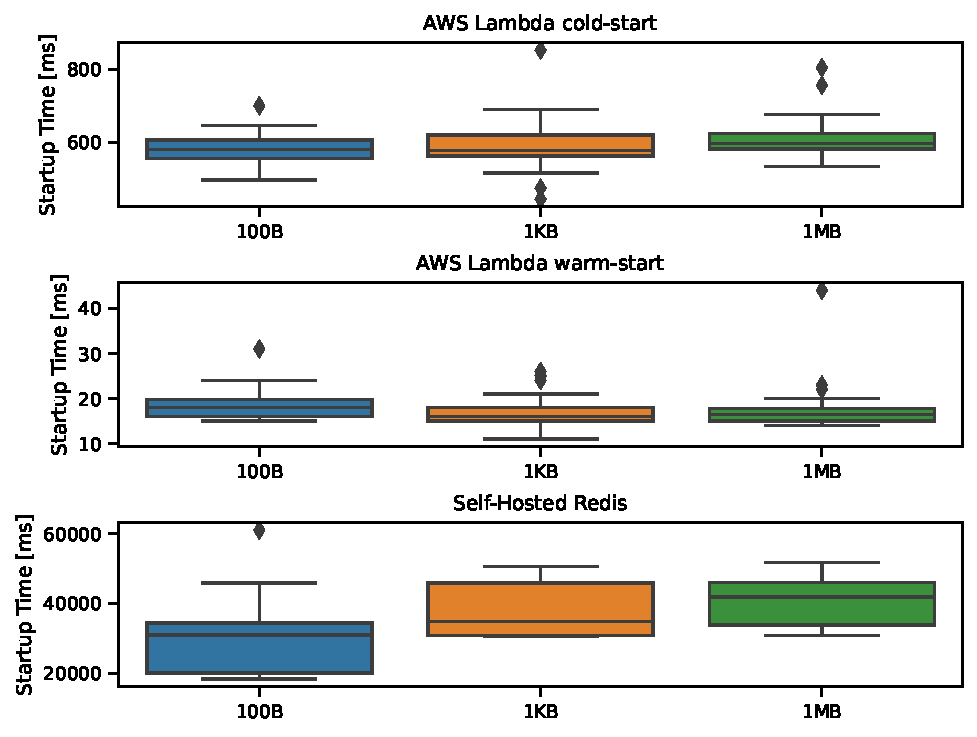
\includegraphics[width=0.8\textwidth]{figures/startup.pdf}
        \caption{Startup latency for the self-hosted Redis layer and the AWS Lambda function divided into cold and warm startups. Each experiment includes 30 measurements, and we also test different object sizes.}
        \label{fig:startup}
    \end{center}
\end{figure}
